\section{Problems Encountered}
\label{sec:problems}
The development of this algorithm has encountered a number of important problems that affected its progress.

Some edge-cases still remain unresolved. For example, Figure \ref{fig:edge} shows a frequently appearing one: the blue guard is stuck on the vertex because its movement direction cannot be projected inside the polygon. So, it cannot move downwards and is instead stuck on the vertex.

\begin{figure}[h!]
    \centering
    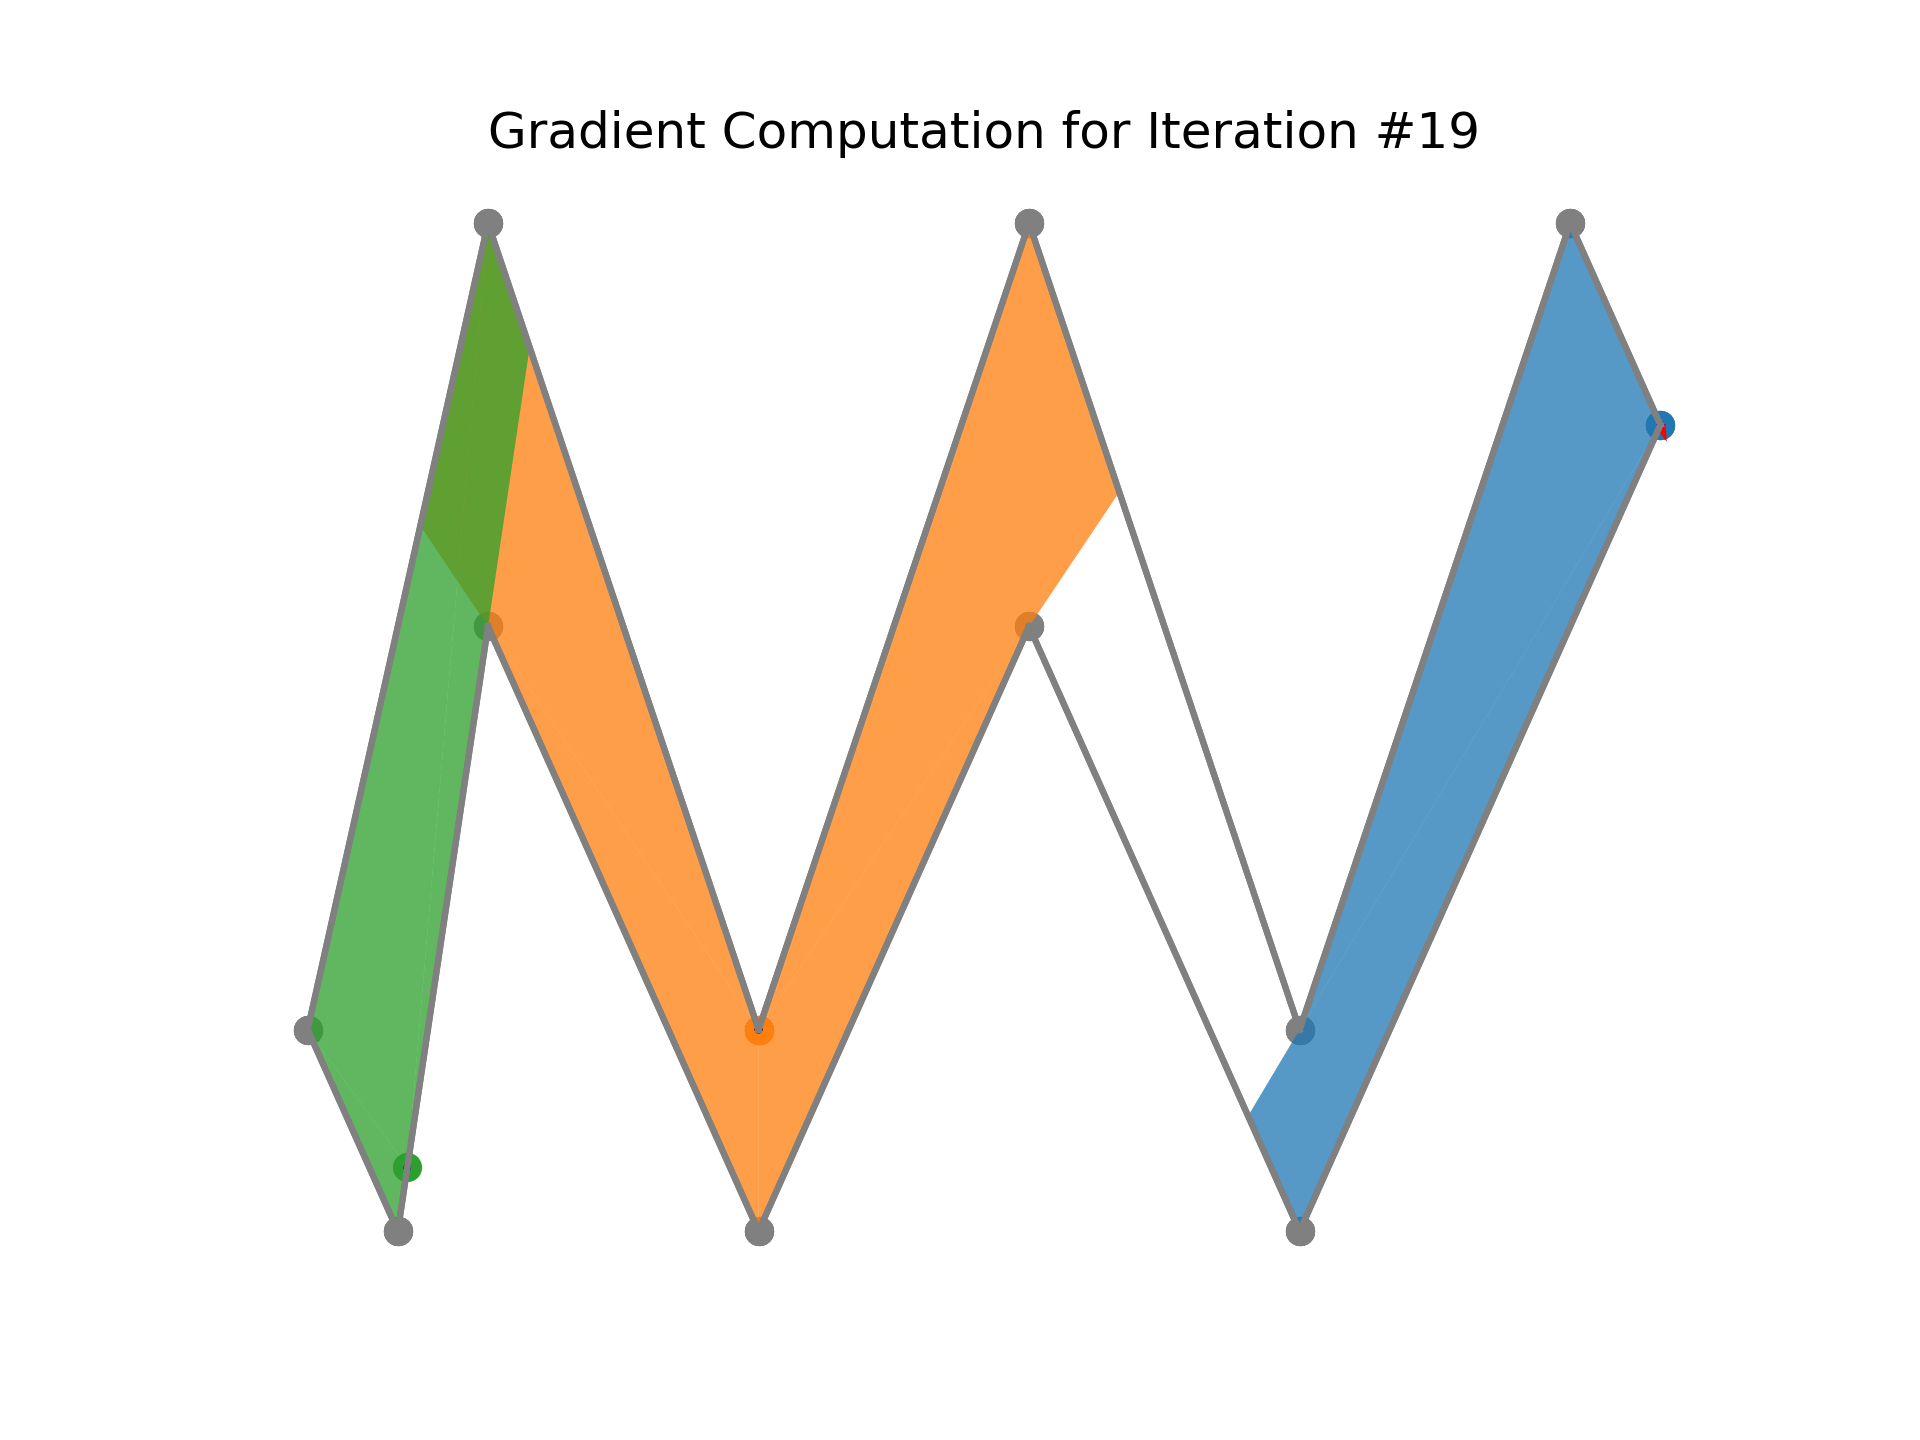
\includegraphics[width = 0.6\textwidth]{experiments/edge_case.png}
    \caption{Edge case for when the blue guard cannot move because its movement direction cannot be projected into a useful direction inside the polygon.}
    \label{fig:edge}
\end{figure}

Moreover, numerous issues were posed by the CGAL library itself, due to its non-detailed errors and lack of explicit documentation. Having to reverse engineer and delve into the source-code of CGAL slowed down the debugging process. Because some errors were not explicit at all, some crashes remained unsolved (for example, the program crashes for certain starting positions for different polygons). Additionally, because of the way CGAL handles number types, we frequently encountered approximation errors. For instance, some guards ``close enough'' to reflex vertices were considered to be on the reflex vertex, even if they were not. Conversely, comparing point coordinates would not always work. So sometimes guards with the same coordinates would not be considered to be overlapping.
As such, the algorithm is thus sensitive to the heuristics used, the shape of the polygons and the values of the hyperparameters. In the Section \ref{sec:experiments} we have mentioned some shapes of polygons that the algorithm can solve, the hyperparameters used and the initial guard positions.
% Some of the polygons the algorithm can solve under the tested circumstances include those mentioned in Section \ref{sec:experiments}. 
We were especially interested in the irrational guards polygon \cite{abrahamsen2021art}. However, the irrational guards polygon can only be solved if the guards are already very close to the optimum. Due to a mysterious CGAL error, we could not fix this issue.
The same vague issue happens with polygons from the APGlib library \cite{art-gallery-instances-page}. In some rare tested polygons the program only got stuck (not crashed). The APGlib library offers an extensive testbed for polygons. So, the fact that we could not address the CGAL error in this thesis' time constraints was quite dissatisfying.

Another problem worth mentioning is scalability. The program does not scale. As mentioned in Section \ref{sec:experiments}, for comb polygons with more than 6 teeth, the waiting time already exceeds an hour to finish. We believe that this waiting time is inadequate for the size and number of guards of the polygon.
Some of the largest bottlenecks that work against scalability are the visibility area and the Hidden Gradient computations. Currently, the visibility area of each guard is updated at every iteration. We are using the Triangular Expansion Visibility \cite{DBLP:journals/corr/BungiuHHHK14} which runs in $O(n)$ time, with $n$ the number of guards. Thus, the visibility computation per iteration runs in $O(n^2)$ time. 
In terms of the Hidden Gradient computation, each guard has its gradient recomputed at most $n$ times. This happens in the case when only one guard out of the $n$ guards has a non-zero gradient, and thus it gets removed from the set. The remaining $n - 1$ guards have their gradient recomputed. Again, in the worst case only one guard has a non-zero gradient. Thus, a guard gets its gradient recomputed in $O(n^2)$ time.
Other poorly scalable parts of the algorithm are based on the number of reflex vertices. The gradient computation depends on the number of reflex vertices $R$. If $R >> n$, then the algorithm will perform poorly for polygons with significantly fewer guards than reflex vertices.

% - cryptic CGAL errors
% - can only work with simple polygons
% - except for the few test polygons (2 guards, random, comb), all the other testbeds (Simon's) don't work because the algorithm gets stuck/crashes
% - for bigger polygons (more guards) it becomes slow very fast (unfeasible)
% - initial guard placement
